\chapter{Implementation of Evolution Scenarios}
This chapter describes implementation details for realizing the Docker environment \ref{DockerImplementation}, the Mobile App Client  for the existing hybrid cloud-based variant of CoCoME (\ref{AppImplementation}) and the Microservice-based variant (\ref{MicroserviceImplementation}).


\section{Using a Docker Environment}\label{DockerImplementation}
 	As shown in Fig. \ref*{Deploym_CoCoME}, the docker Container contains five different Glassfish servers. In particular they are called \textit{WEB}, \textit{ENTERPRISE}, \textit{STORE}, \textit{REGISTRY} and \textit{ADAPTER}. By default, Glassfish provides a Derby DB that is connected to the Service Adapter using Java Database Conectivity (JDBS) interface.
 	\begin{figure}[h]
 		\centering
 		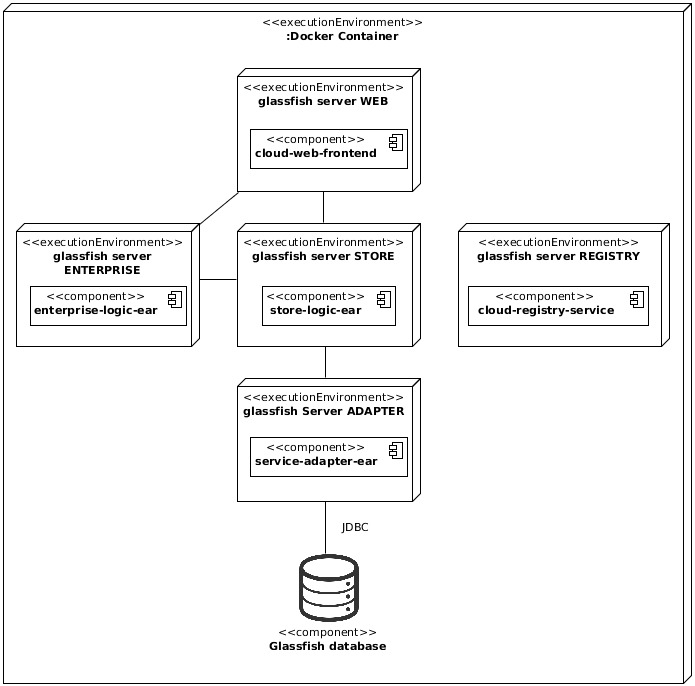
\includegraphics[width = 0.8\textwidth]{img/docker_Container_Deployment.png}
 		\caption{Deployment diagram CoCoME}
 		\label{Deploym_CoCoME}
 	\end{figure}
 	
 	The deployment assignment within the Docker environment is identical to the one specified in CoCoME deployment guide.
 	This means the maven generated archive files \textit{cloud-web-frontend},\textit{enterprise-logic-ear},\textit{store-logic-ear}\textit{cloud-registry-sevice} and \textit{service-adapter-ear} are deployed on the servers by using the following assignment:
 	\begin{figure}[H]
 		\centering
 		\begin{tabular}{p{0.25\textwidth}|p{0.01\textwidth}p{0.25\textwidth}}
 			Server && Deployment file \\
 			\hline
 			WEB && cloud-web-frontend  \\
 			ENTERPRISE && enterprise-logic-ear  \\
 			STORE && store-logic-ear  \\
 			REGISTRY && cloud-registry-service  \\
 			ADAPTER && service-adapter-ear \\	
 		\end{tabular}
 		\caption{Assignment of archive files to Servers}
 		\label{table_assignment}
 	\end{figure}
    As mentioned earlier, there are two versions of this Docker project.\\
 	 The fast version can be extended by the Pick-Up shop\footnote{\url{https://github.com/cocome-community-case-study/cocome-cloud-jee-web-shop}}. This Pick-Up shop runs inside a separate Docker container which is shown in figure \ref{Deploym_Pickup}.  
 	\begin{figure}[h]
 		\centering
 		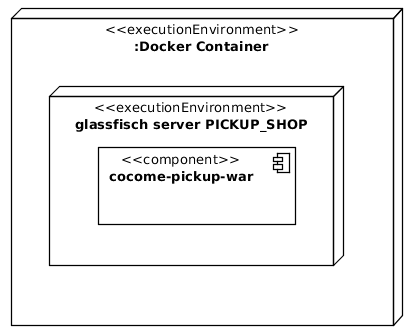
\includegraphics[width = 0.4\textwidth]{img/docker_Container_PickUP.png}
 		\caption{Deployment diagram CoCoME Pickup Shop}
 		\label{Deploym_Pickup}
 	\end{figure}
 	As shown in figure \ref*{Deploym_Pickup}, this container provides only one Glassfish server.
 	\begin{figure}[H]
 		\centering
 		\begin{tabular}{p{0.25\textwidth}|p{0.01\textwidth}p{0.25\textwidth}}
 			Server && Deployment file \\
 			\hline
 			PICKUP\_SHOP && cocome-pickup-war \\	
 		\end{tabular}
 		\caption{Assignment archive files to Servers}
 		\label{table_assignment_pickup}
 	\end{figure}
 	To control the start of both containers, precisely the CoCoME and the Pick-Up Shop, another specific file is needed: the Docker Compose file. It ensures that the CoCoME Container is active, before the Pick-Up Shop container starts. This is necessary as the Pickup Shop requires a running instance of CoCoME to register itself.\\
 	Whereas CoCOME does not require the Pick-Up Shop, the inversion is not corrext.
 	Both containers need to communicate with each other. By default, docker prohibits any outgoing and ingoing communication from and in a container. This is solved by opening specific ports through which the communication is possible. Which ports the containers can use is specified in the Docker Compose file as well.
 	
 	
 \section{Adding a Mobile App Client}\label{AppImplementation}
Adding a Mobile App Client did not require a modification within the hybrid cloud-based variant of CoCoME. The implementation was done using the Cordova framework and OnsenUI to provide a multi OS compatible backend and UI \cite{schnabel}. The App itself is written in Typescript/Javascript. Fig. \ref{App_ClassDiagram} shows the principal classes and their relationships.
\\
The \textit{Navigator} is the primary class that manages the pages. The pages consist of two components: The \textit{Page} itself and its \textit{PageState}. The \textit{PageState} is used to store and transfer the current status of a page. There are currently six different pages available: \textit{IndexPage}, \textit{SearchPage}, \textit{ItemPage}, \textit{CheckoutPage}, \textit{CartPage} and \textit{LoginPage}. For the sake of clarity, they are subsumed under the generic terms \textit{ConcretePage} and \textit{ConcretePageState}. 
\\
Pages use components. Such components are i.e. the \textit{Navbar} or the \textit{Searchbar}. These components are abstract descriptions of UI elements that are connected to the actual \textit{HTML-elements} via Knockout.js. By using Knockout.js, changing values of a component results in an immediate change of the UI. 
Besides, the App Client retrieves information of the CoCoME system.  As mentioned in \ref{DesignMobileApp}, the Client is not able to access the CoCoME system directly. Therefore, the pages use \textit{Services} provided by a \textit{ServiceHolder} to call the \textit{AppController'} Rest-API. The \textit{AppController} is written in Java using the SpringBoot framework and converts the Rest-requests of the App Client to SOAP-Requests in order to match the CoCoME-API. 
  
  
   \begin{sidewaysfigure}[ht]
  	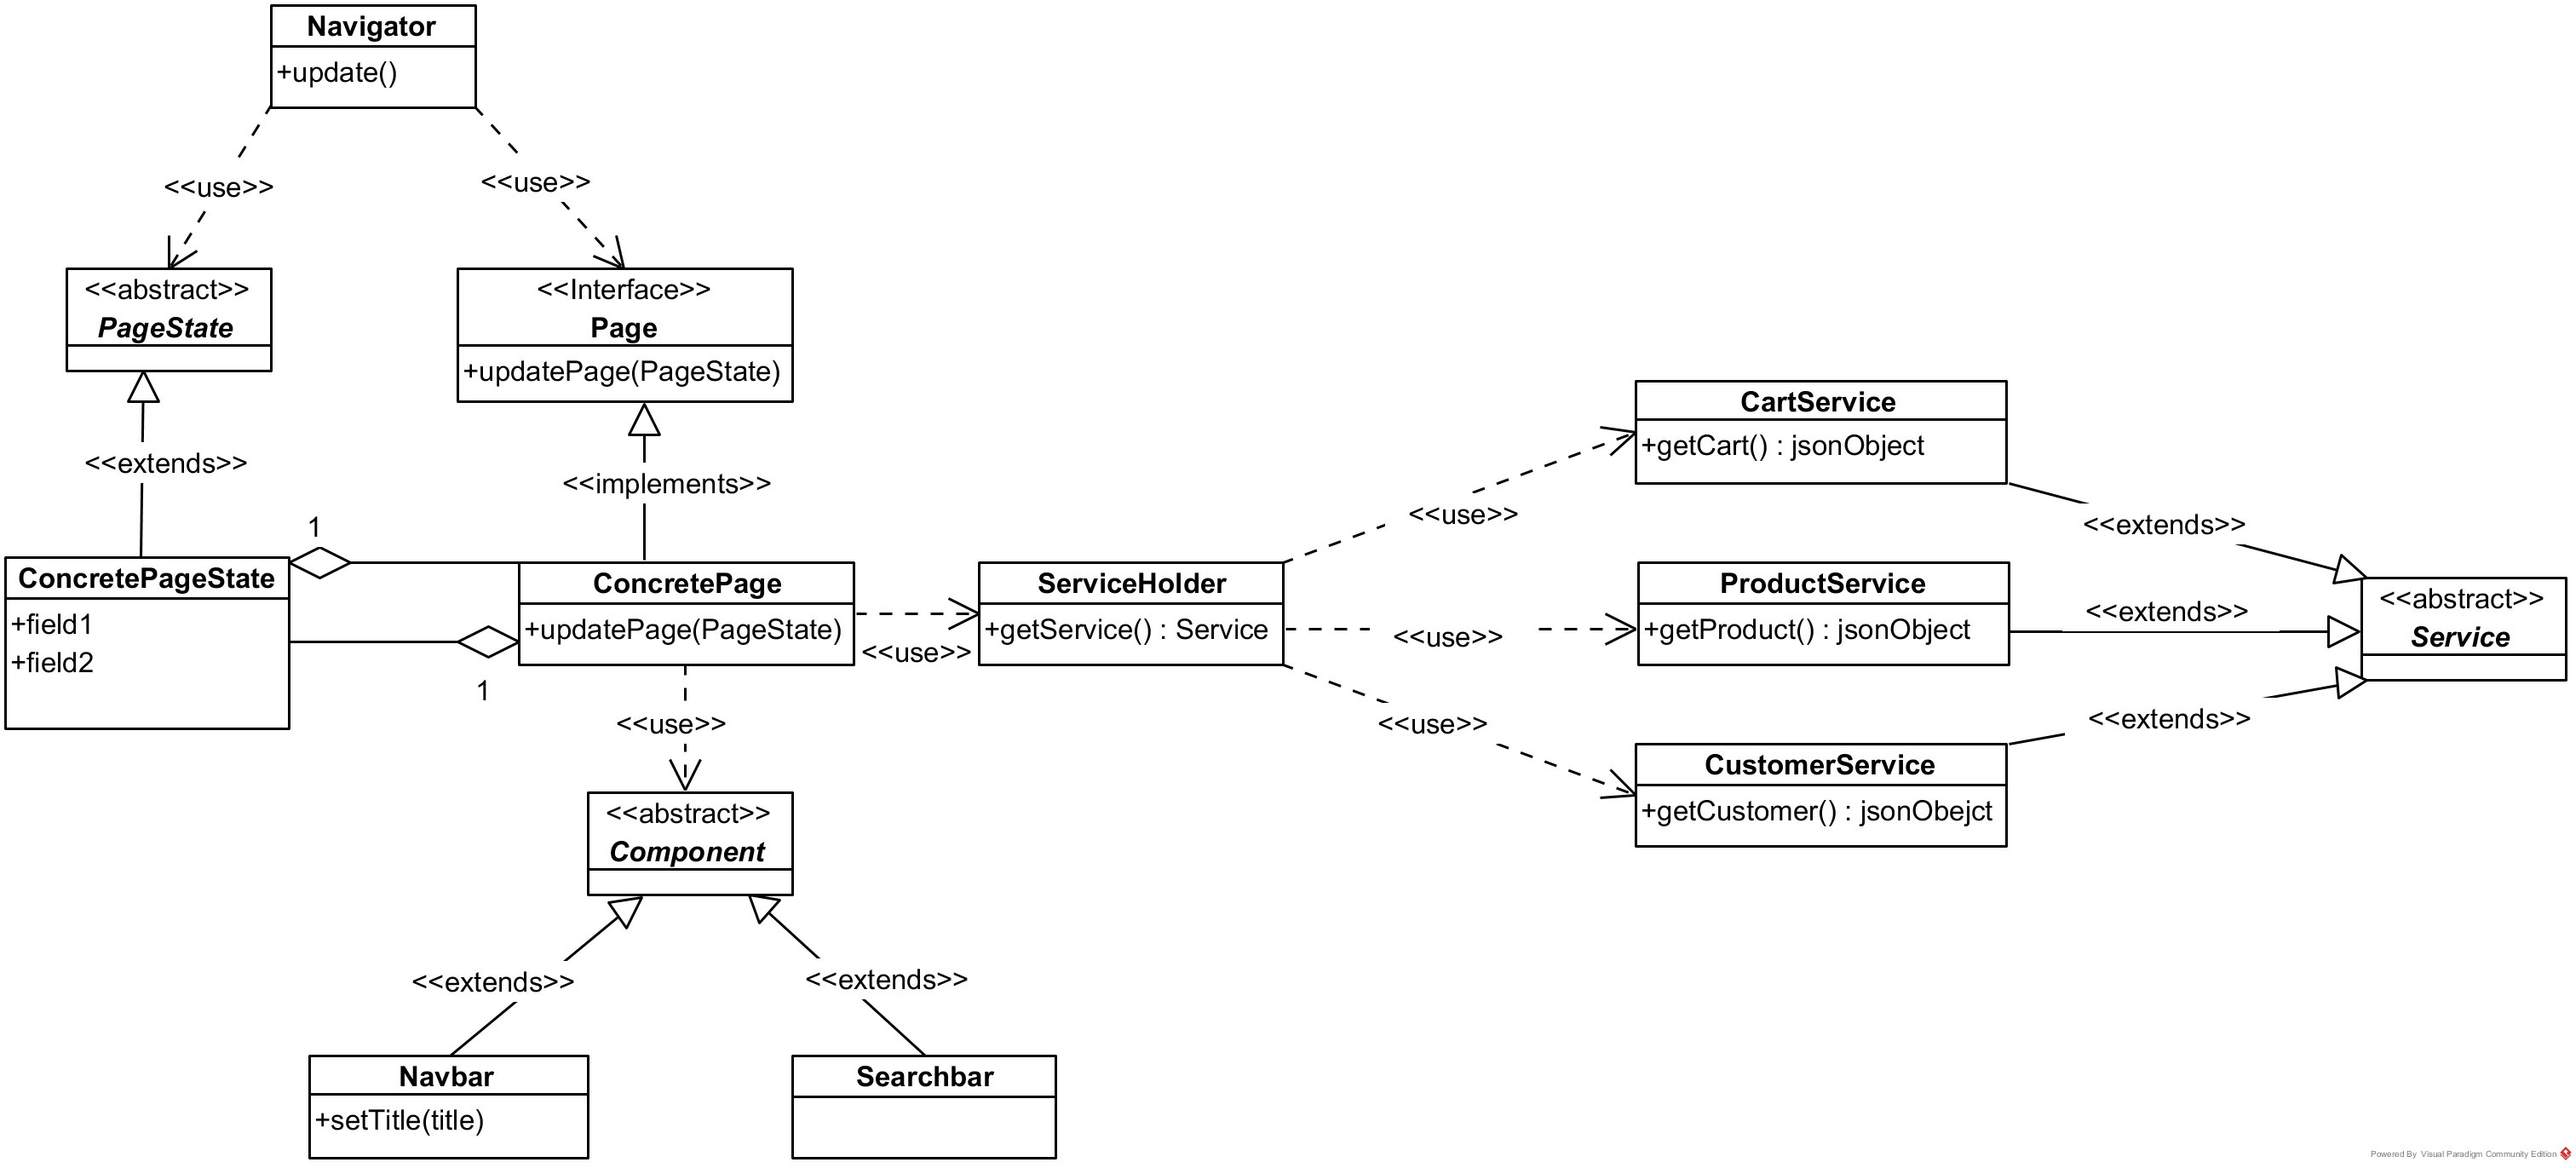
\includegraphics[width=\textwidth]{img/appBasicClass.png}
  	\caption{Primary Classes of the App}
  	\label{App_ClassDiagram}
  \end{sidewaysfigure}

\FloatBarrier
 
 
 \section{Using Microservice Technology} \label{MicroserviceImplementation}
 The CoCoME microservice evolution scenario transfers the functionality of original CoCoME Plain Java variant into microservices by implementing an microservice architecture and using rest communication. The implementation was done using Eclipse for Java and Glassfish to deploy the applications. Further, the Java Persistence API is used for persisting and mapping Java classes to structures of relational databases. JAX-RS offers functionality for recourse oriented WEB-APIs based on REST-Architectural style. JAXB defines an interface for serialize and deserialize of JAVA-classes to XML- or JSON-files. 
 \\
 As can be seen in figure \ref{projectStructure} each service project contains three sub-projects, namely \textit{name}-service-ejb, \textit{name}-service-rest and \textit{name}-service-ear. The first one contains the logical implementation of these projects as well as the functionality for persisting the  second provides the rest implementation. Also it has via injections access to the database. The last one is used for packaging the projects to ear files. 
 
	\begin{figure}[h]
		\centering
		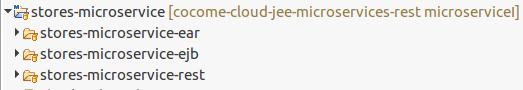
\includegraphics[width = 0.8\textwidth] {img/projectStructure_Micro.png}
	 	\caption{Project structure microservices}[The structure shown in in this figure is implemeted in the same way for the other microservices.]
	 	\label{projectStructure}
	 	
 	\end{figure}
 	
